\chapter{Resultados y Pruebas} \label{sec:Resultados}

En cada ciclo de prueba se modificó únicamente el CNI bajo evaluación; hardware, sistema operativo, versión de Kubernetes, tamaño de paquetes, duración y condiciones de red permanecieron constantes, lo que hace posible atribuir las diferencias observadas al plugin y no al entorno.

\section{Metodología General de Pruebas}

\subsection{Control de Condiciones: el Escenario de Referencia}

Se definió un escenario de referencia con los siguientes parámetros fijos para todos los CNIs:

\begin{table}[htbp]
\centering
\scriptsize
\caption{Parámetros del escenario de referencia para todas las pruebas.}
\label{tab:baseline-pruebas}
\begin{tabularx}{\textwidth}{|Y|Y|}
\hline
\textbf{Parámetro Controlado} & \textbf{Valor Fijo para Todo el Experimento} \\
\hline
Tipo de instancia cloud & DigitalOcean Droplet --- Ubuntu 22.04 LTS, 2 vCPU, 4 GB RAM para nodos Worker \\
\hline
Versión de Kubernetes & K3s canal stable --- la misma versión en todos los ciclos de prueba \\
\hline
Región del datacenter & nyc3 (Nueva York) --- mismo datacenter para todos los nodos en todas las pruebas \\
\hline
Red entre nodos & VPC privada DigitalOcean --- MTU 1500 bytes, sin tráfico externo \\
\hline
Duración de cada prueba iperf3 & 300 segundos (5 minutos) por corrida \\
\hline
Número de corridas por CNI & 5 corridas independientes --- permite calcular promedios y detectar variabilidad \\
\hline
Protocolo de red bajo prueba & TCP --- el protocolo dominante en aplicaciones empresariales reales \\
\hline
Herramienta de throughput & iperf3 con salida JSON (\texttt{-J}), un solo stream TCP (\texttt{-P 1}) \\
\hline
Herramienta de latencia & Script Bash con \texttt{nc -z -w 2} --- 30 muestras por corrida \\
\hline
\end{tabularx}
\end{table}

\subsection{Automatización: de la Prueba Manual a la Prueba Orquestada}

Todas las pruebas se orquestaron mediante CronJobs de Kubernetes. La secuencia de ejecución automática en cada ciclo fue:
\begin{enumerate}
\item CronJob del cliente iperf3 se activa (minutos 0 y 30). Kubernetes crea el Pod cliente en un nodo diferente al servidor (podAntiAffinity suave, weight 100).
\item Pod cliente ejecuta iperf3 durante 300 segundos y guarda el resultado JSON.
\item CronJob del cliente de latencia ejecuta 30 mediciones de TCP connect (minutos 10 y 40) y guarda su resultado JSON.
\item Al finalizar ambas pruebas, el Resource Usage Exporter (minutos 25 y 55) consulta Prometheus para extraer el consumo de CPU y RAM del agente CNI.
\item \texttt{procesador.js} actualiza \texttt{cni-data.json} con los nuevos datos procesados.
\end{enumerate}

La orquestación automática elimina la variabilidad humana de la ejecución: cada corrida sigue exactamente la misma secuencia con los mismos intervalos, de modo que las diferencias observadas entre CNIs se deben al plugin y no al operador.

La elección de cinco corridas por CNI responde a un equilibrio entre rigor estadístico y viabilidad operativa. Una sola corrida permitiría que un dato atípico o evento anómalo dominara el resultado, mientras que un número muy elevado extendería el tiempo de prueba sin un beneficio proporcional. Con cinco corridas distribuidas en el tiempo, el algoritmo IQR puede identificar y descartar una corrida anómala, y el promedio de las restantes resulta estadísticamente representativo; este criterio es habitual en la investigación de redes sobre entornos cloud \cite{ref7,ref8}.

\section{Pruebas de Rendimiento de Red --- Objetivo Específico 1}

\subsection{Protocolo de Prueba de Throughput con iperf3}

iperf3 establece una conexión entre un proceso servidor y un proceso cliente, y el cliente envía datos lo más rápido que la red permite durante el tiempo configurado. Se usó el parámetro \texttt{-P 1} (un solo stream TCP) para representar el comportamiento de una aplicación empresarial típica, no la carga máxima teórica.

\begin{lstlisting}
# Comando iperf3 ejecutado por el CronJob cliente
# -c: servidor  -t: 300s  -J: JSON  -P 1: un solo stream
iperf3 -c iperf-server-svc.cni-benchmark.svc.cluster.local \
  -t 300 -J -P 1 \
  > /results/throughput-$(date +%Y%m%d_%H%M%S)-${CNI_NAME}.json
\end{lstlisting}

\subsection{Resultados de Throughput TCP por CNI}

Los resultados presentados son los promedios de las 5 corridas de 300 segundos para cada CNI, después de aplicar el filtro IQR para eliminar outliers. La Tabla~\ref{tab:throughput-resultados} registra tres dimensiones de calidad del canal: cuántos datos por segundo puede transportar (throughput), cuántos paquetes tuvieron que reenviarse por error (retransmisiones) y qué tan predecible es el canal entre corridas (variabilidad).

\begin{table}[htbp]
\centering
\scriptsize
\caption{Resultados de rendimiento TCP por CNI (promedio de 5 corridas de 300 segundos, outliers IQR eliminados).}
\label{tab:throughput-resultados}
\begin{tabularx}{\textwidth}{|Y|c|c|c|c|}
\hline
\textbf{Métrica} & \textbf{Flannel (VXLAN)} & \textbf{Calico (VXLAN)} & \textbf{Cilium (eBPF)} & \textbf{Antrea (OVS)} \\
\hline
Throughput promedio --- Mbps \newline\textit{($\uparrow$ mayor es mejor: más datos por segundo)} & 1452.97 & \textbf{1804.40} & 843.56 & 1588.45 \\
\hline
Retransmisiones TCP --- paquetes/sesión \newline\textit{($\downarrow$ menor es mejor: menos retransmisiones en el canal)} & \textbf{11774} & 68993 & 15142 & 42229 \\
\hline
Outliers descartados (Throughput) & 0 de 5 (0\%) & 0 de 5 (0\%) & 1 de 5 (20\%) & 0 de 5 (0\%) \\
\hline
Outliers descartados (Retransmisiones) & 0 de 5 (0\%) & 1 de 5 (20\%) & 0 de 5 (0\%) & 0 de 5 (0\%) \\
\hline
\end{tabularx}
\end{table}

A diferencia de los entornos locales de alto rendimiento, la red en nube VPC privada de DigitalOcean limita el ancho de banda efectivo, registrándose valores máximos de throughput de 1804.40 Mbps en Calico, seguido de Antrea con 1588.45 Mbps y Flannel con 1452.97 Mbps. Cilium presenta el valor más bajo con 843.56 Mbps. Las diferencias en retransmisiones TCP son críticas: Flannel destaca con la menor cantidad de retransmisiones (11774), seguido por Cilium (15142) y Antrea (42229), mientras que Calico registra la tasa de fallas más alta con 68993 retransmisiones. Esto indica que a pesar de que Calico lidera el throughput bruto, genera un mayor estrés de reenvío de paquetes debido a la saturación del datapath.

\subsection{Protocolo de Prueba de Latencia TCP}

La latencia reportada en este experimento no mide el tiempo de tránsito físico puro de la red (latencia de enlace L3/L4 intra-VPC, habitualmente inferior a 1 ms), sino el tiempo total de establecimiento de conexión TCP a nivel de aplicación. El cliente ejecuta un \emph{script} Bash iterando \texttt{nc -z -w 2} hacia el servicio \texttt{iperf3-server}, lo que captura no solo el \emph{handshake} de tres vías, sino el overhead del \emph{spawn} del proceso en el sistema operativo y la resolución DNS interna de Kubernetes en cada ciclo. Esta métrica de latencia final (12-35 ms) resulta útil para comparar el estrés relativo que cada CNI impone al stack de red bajo este tipo de rutinas de microservicios, pero los valores absolutos no deben interpretarse como la latencia base de la red virtual de DigitalOcean.

\subsection{Resultados de Latencia TCP por CNI}

En todas las filas de la Tabla~\ref{tab:latencia-resultados}, \textbf{un valor menor es mejor ($\downarrow$)}: menos milisegundos significa que el CNI establece conexiones más rápido. La latencia máxima refleja el comportamiento bajo condiciones adversas de carga de red, mientras que el Jitter (MDEV) mide la predictibilidad del enlace.

\begin{table}[htbp]
\centering
\scriptsize
\caption{Resultados de latencia TCP por CNI (30 muestras $\times$ 5 corridas, outliers IQR eliminados). Todas las métricas: $\downarrow$ menor es mejor.}
\label{tab:latencia-resultados}
\begin{tabularx}{\textwidth}{|Y|c|c|c|c|}
\hline
\textbf{Métrica de Latencia ($\downarrow$ menor=mejor)} & \textbf{Flannel (VXLAN)} & \textbf{Calico (VXLAN)} & \textbf{Cilium (eBPF)} & \textbf{Antrea (OVS)} \\
\hline
Latencia promedio --- ms \newline\textit{(comportamiento típico)} & 21.53 & \textbf{12.54} & 18.73 & 35.09 \\
\hline
Latencia máxima --- ms \newline\textit{(peor caso observado)} & 50.80 & \textbf{44.20} & 47.00 & 83.50 \\
\hline
Jitter (MDEV) --- ms \newline\textit{(variabilidad de la latencia)} & 7.76 & \textbf{7.31} & 8.47 & 17.25 \\
\hline
Outliers descartados (Latencia Max) & 0 de 5 (0\%) & 0 de 5 (0\%) & 0 de 5 (0\%) & 1 de 5 (20\%) \\
\hline
\end{tabularx}
\end{table}

Los datos de latencia revelan la mayor brecha de rendimiento entre CNIs. Calico logra la menor latencia promedio (12.54 ms) y el menor jitter (7.31 ms). Cilium se sitúa en segundo lugar con una latencia promedio de 18.73 ms, seguido por Flannel con 21.53 ms. Antrea registra el desempeño más bajo, alcanzando una latencia promedio de 35.09 ms y un jitter elevado de 17.25 ms (más del doble que Calico). Esto indica que para entornos donde el tiempo de establecimiento de conexión TCP es un factor de éxito (como APIs web interactivas), Calico ofrece la respuesta más rápida y estable.

\section{Pruebas de Seguridad con Network Policies --- Objetivo Específico 2}

\subsection{Matriz de Pruebas de Network Policies}

Se diseñó una matriz de pruebas que cubre los escenarios críticos de seguridad en un clúster Kubernetes. La herramienta de verificación principal fue \texttt{kubectl exec} combinada con \texttt{nc} (netcat) dentro de Pods de prueba.

\begin{table}[htbp]
\centering
\scriptsize
\caption{Matriz completa de pruebas de seguridad con Network Policies.}
\label{tab:matriz-seguridad}
\begin{tabularx}{\textwidth}{|Y|Y|}
\hline
\textbf{Caso de Prueba} & \textbf{Descripción, Herramienta y Criterio de Éxito} \\
\hline
TC-SEC-01: Default Deny Ingress & Ningún Pod externo puede enviar tráfico al namespace sin regla explícita. Verificación: \texttt{nc -zv <pod-ip> 8080}. ÉXITO: timeout en menos de 5 s. \\
\hline
TC-SEC-02: Default Deny Egress & Los Pods en producción no pueden iniciar conexiones salientes no autorizadas. Verificación: \texttt{curl --max-time 3}. ÉXITO: timeout. \\
\hline
TC-SEC-03: Frontend$\rightarrow$Backend permitido & Pod con etiqueta \texttt{tier=frontend} puede conectarse al backend en puerto 8080. ÉXITO: Connection succeeded. \\
\hline
TC-SEC-04: Bloqueo Frontend$\rightarrow$Database & Pod frontend NO puede conectarse a la base de datos directamente. ÉXITO: Connection refused o timeout. \\
\hline
TC-SEC-05: Backend$\rightarrow$Database permitido & Pod backend SÍ puede conectarse a la base de datos en puerto 5432. ÉXITO: Connection succeeded. \\
\hline
TC-SEC-06: Database NO inicia conexiones & La base de datos nunca inicia conexiones salientes. ÉXITO: Bloqueo por política de Egress. \\
\hline
TC-SEC-07: Bloqueo entre namespaces & Un Pod de namespace staging no puede comunicarse con Pods de production. ÉXITO: Bloqueo confirmado. \\
\hline
TC-SEC-08: GitOps Auto-restauración & Si una política se elimina manualmente, ArgoCD la restaura en menos de 3 minutos. ÉXITO: Política restaurada automáticamente. \\
\hline
\end{tabularx}
\end{table}

\subsection{Resultados de las Pruebas de Seguridad por CNI}

\begin{table}[htbp]
\centering
\scriptsize
\caption{Resultados de pruebas de seguridad por CNI.}
\label{tab:resultados-seguridad}
\begin{tabularx}{\textwidth}{|Y|Y|Y|Y|Y|}
\hline
\textbf{Caso de Prueba} & \textbf{Flannel} & \textbf{Calico} & \textbf{Cilium} & \textbf{Antrea} \\
\hline
TC-SEC-01: Default Deny Ingress & NO SOPORTA & PASA & PASA & PASA \\
\hline
TC-SEC-02: Default Deny Egress & NO SOPORTA & PASA & PASA & PASA \\
\hline
TC-SEC-03: Frontend$\rightarrow$Backend & N/A & PASA & PASA & PASA \\
\hline
TC-SEC-04: Frontend$\rightarrow$DB bloqueado & NO BLOQUEA & PASA & PASA & PASA \\
\hline
TC-SEC-05: Backend$\rightarrow$DB permitido & N/A & PASA & PASA & PASA \\
\hline
TC-SEC-06: DB no inicia conexiones & NO SOPORTA & PASA & PASA & PASA \\
\hline
TC-SEC-07: Bloqueo entre namespaces & NO BLOQUEA & PASA & PASA & PASA \\
\hline
TC-SEC-08: Auto-restauración ArgoCD & N/A & PASA ($<$2 min) & PASA ($<$2 min) & PASA ($<$2 min) \\
\hline
Network Policies L7 (HTTP paths) & NO SOPORTA & NO SOPORTA & SOPORTA & NO SOPORTA \\
\hline
\textbf{RESULTADO GLOBAL} & \textbf{INSUFICIENTE} & \textbf{APROBADO} & \textbf{APROBADO+} & \textbf{APROBADO} \\
\hline
\end{tabularx}
\end{table}

El hallazgo más crítico es que Flannel no implementa Network Policies en su plano de datos: las políticas se crean sin error en Kubernetes, pero el tráfico que debería bloquearse continúa fluyendo. Esto descarta a Flannel para cualquier organización con requisitos de seguridad.

Cilium es el único CNI que soporta Network Policies de capa 7 (L7), lo que permite definir reglas a nivel de método y ruta HTTP ---por ejemplo, admitir solo solicitudes \texttt{GET} a una ruta determinada---, capacidad fundamental para arquitecturas de microservicios.

\subsection{Prueba de Overhead de Seguridad}

Se ejecutaron las pruebas de rendimiento nuevamente con las políticas de seguridad activas y se compararon con los resultados base. El \textbf{overhead} es el costo adicional que introduce activar las políticas: \textbf{cuanto menor el porcentaje, mejor ($\downarrow$)}, porque significa que la seguridad se aplica sin penalizar el rendimiento de las aplicaciones. Un overhead del 5\% en latencia, por ejemplo, significa que una conexión que tardaba 0.500\,ms ahora tarda 0.525\,ms --- imperceptible para el usuario final.

\begin{table}[htbp]
\centering
\scriptsize
\caption{Porcentaje de overhead (impacto negativo) introducido al activar Network Policies por escenario.}
\label{tab:overhead-seguridad}
\begin{tabularx}{\textwidth}{|Y|c|c|c|}
\hline
\textbf{CNI} & \textbf{Zero Trust (Overhead)} & \textbf{Multi-Tier (Overhead)} & \textbf{Egress Block (Overhead)} \\
\hline
\textbf{Calico} & Thr: $-$0.25\% / Lat: $-$21.11\% & Thr: $-$0.25\% / Lat: $+$31.45\% & Thr: $-$1.36\% / Lat: $-$22.25\% \\
\hline
\textbf{Cilium} & Thr: $+$111.53\% / Lat: $-$43.16\% & Thr: $+$92.07\% / Lat: $+$3.70\% & Thr: $+$108.05\% / Lat: $-$37.43\% \\
\hline
\textbf{Antrea} & Thr: $+$4.40\% / Lat: $-$28.77\% & Thr: $+$13.46\% / Lat: $-$25.16\% & Thr: $-$4.35\% / Lat: $-$27.15\% \\
\hline
\textbf{Flannel} & \multicolumn{3}{c|}{No soporta Network Policies nativas (Capacidad 0/10)} \\
\hline
\end{tabularx}
\end{table}

El impacto de habilitar políticas de seguridad varía considerablemente. Calico muestra un impacto mínimo en throughput (menos del 1.36\% de pérdida) con variaciones de latencia de entre un $-22.25\%$ (reducción) y un $+31.45\%$ (incremento). Antrea registra incrementos de throughput de hasta $+13.46\%$ y reducciones de latencia de hasta $-28.77\%$. En el caso de Cilium, se observa una anomalía estadística: el rendimiento de red aparente mejora notablemente al habilitar políticas (el throughput aumenta un $+111.53\%$). Sin embargo, este salto porcentual no significa que las políticas L7 aceleren la red por sí mismas, sino que evidencia un \emph{baseline} subóptimo en este testbed ---posiblemente afectado por ruido de monitoreo o el desajuste inicial de MTU derivado del encapsulamiento VXLAN y eBPF--- que se estabiliza al activar el filtrado explícito. Por consiguiente, esta mejora relativa no debe generalizarse como un comportamiento estándar en entornos de producción. Flannel no registra datos al no poder compilar o aplicar políticas de seguridad en su plano de datos.

\section{Pruebas de Eficiencia Computacional --- Consumo del Agente CNI}

Las métricas de consumo fueron capturadas por Prometheus durante las sesiones activas de iperf3 (cuando la red estaba bajo carga máxima). Se midió específicamente el consumo del proceso del agente CNI en cada nodo Worker. En esta tabla conviven dos direcciones de optimización: \textbf{CPU y RAM son mejores cuanto menores sean ($\downarrow$)}, porque el CNI consume recursos que de otro modo estarían disponibles para las aplicaciones; la \textbf{eficiencia Gbps/100\,m es mejor cuanto mayor sea ($\uparrow$)}, porque indica cuánto tráfico puede procesar el CNI por cada unidad de CPU que consume. Un millicore (m) equivale a la milésima parte de un núcleo de CPU: 1\,000\,m = 1 núcleo completo.

\begin{table}[htbp]
\centering
\scriptsize
\caption{Consumo computacional promedio del agente CNI bajo estrés de red (tráfico TCP intenso).}
\label{tab:consumo-recursos}
\begin{tabularx}{\textwidth}{|Y|c|c|c|c|}
\hline
\textbf{Métrica de Eficiencia} & \textbf{Flannel (VXLAN)} & \textbf{Calico (VXLAN)} & \textbf{Cilium (eBPF)} & \textbf{Antrea (OVS)} \\
\hline
Nombre del agente CNI & flanneld & calico-node & cilium-agent & antrea-agent \\
\hline
Uso de CPU promedio --- \% del nodo \newline\textit{($\downarrow$ menor es mejor)} & \textbf{19.45\%} & 29.05\% & 25.79\% & 27.75\% \\
\hline
Uso de RAM promedio --- MB \newline\textit{($\downarrow$ menor es mejor)} & \textbf{1176.54 MB} & 1672.83 MB & 1497.19 MB & 1429.95 MB \\
\hline
\end{tabularx}
\end{table}

Los resultados de consumo revelan que Flannel es el CNI más liviano en el host, consumiendo solo un 19.45% de CPU del nodo y 1176.54 MB de memoria RAM promedio bajo estrés. Por el contrario, Calico registra la huella más pesada con un 29.05% de CPU y 1672.83 MB de RAM. Cilium y Antrea ocupan puestos intermedios, donde Cilium consume un 25.79% de CPU y 1497.19 MB de RAM, y Antrea consume un 27.75% de CPU y 1429.95 MB de RAM. Estos resultados demuestran que el datapath minimalista de Flannel minimiza el costo fijo en hardware, haciéndolo atractivo para clústeres pequeños o con recursos limitados.

\section{Validación del Modelo Matemático MCDA --- Objetivo Específico 3}

\subsection{Validación del Algoritmo IQR}

Para validar que el algoritmo IQR funciona correctamente, se inyectó artificialmente 1 outlier extremo en el conjunto de datos de cada CNI (un valor de latencia 10 veces mayor al promedio real). Se verificó que el IQR lo detectara y excluyera correctamente:

\begin{table}[htbp]
\centering
\scriptsize
\caption{Validación del algoritmo IQR con outlier controlado inyectado artificialmente.}
\label{tab:iqr-validacion}
\begin{tabularx}{\textwidth}{|Y|Y|}
\hline
\textbf{Verificación del IQR} & \textbf{Resultado Observado} \\
\hline
Latencia promedio de Cilium sin outlier & 18.73 ms \\
\hline
Latencia promedio de Cilium CON outlier (sin IQR) & 52.44 ms (+180.0\% de error) \\
\hline
Latencia promedio de Cilium CON outlier y CON IQR & 18.73 ms (0.0\% de error) \\
\hline
¿El IQR detectó el outlier? & SÍ --- el valor 187.30 ms quedó fuera del rango [Q1-1.5$\times$IQR, Q3+1.5$\times$IQR] \\
\hline
Porcentaje de corridas descartadas en datos reales & Entre 0\% y 20\% por CNI \\
\hline
\end{tabularx}
\end{table}

Esta validación confirma que el promedio reportado para cada CNI es robusto ante eventos atípicos del entorno cloud, y que las diferencias entre CNIs en los resultados finales reflejan comportamiento estructural del plugin y no ruido experimental.

\subsection{Validación de la Normalización Min-Max}

La Tabla~\ref{tab:normalizacion-validacion} muestra los valores brutos de cada métrica junto con su equivalente normalizado en la escala 1--5 que utiliza el modelo MCDA. La regla de lectura es uniforme: \textbf{5.00 = mejor CNI en esa dimensión; 1.00 = peor CNI en esa dimensión}, independientemente de las unidades originales (Mbps, ms, \%, MB). Esta escala permite comparar directamente métricas que originalmente tienen magnitudes y unidades muy distintas.

\begin{table}[htbp]
\centering
\scriptsize
\caption{Validación de la normalización min-max de las seis métricas del modelo MCDA (Escala del Recommender: 1.00 = peor, 5.00 = mejor).}
\label{tab:normalizacion-validacion}
\begin{tabularx}{\textwidth}{|Y|c|c|c|c|}
\hline
\textbf{Métrica / Criterio} & \textbf{Flannel} & \textbf{Calico} & \textbf{Cilium} & \textbf{Antrea} \\
\hline
Throughput raw (Mbps) & 1452.97 & 1804.40 & 843.56 & 1588.45 \\
Throughput normalizado (1--5) & 3.54 & \textbf{5.00} & 1.00 & 4.10 \\
\hline
Latencia raw (ms) & 21.53 & 12.54 & 18.73 & 35.09 \\
Latencia normalizada (1--5) & 3.41 & \textbf{5.00} & 3.90 & 1.00 \\
\hline
Retransmisiones raw (por sesión) & 11774 & 68993 & 15142 & 42229 \\
Jitter+Retransmisiones (1--5) & \textbf{4.91} & 3.00 & 4.64 & 1.94 \\
\hline
CPU promedio (\% nodo) & 19.45\% & 29.05\% & 25.79\% & 27.75\% \\
RAM promedio (MB) & 1176.54 & 1672.83 & 1497.19 & 1429.95 \\
Eficiencia de Recursos (1--5) & \textbf{5.00} & 1.00 & 2.39 & 2.25 \\
\hline
Soporte de NetworkPolicies L7 (1--5) & 1.00 & 1.00 & \textbf{5.00} & 1.89 \\
\hline
\end{tabularx}
\end{table}

La tabla de normalización muestra las seis métricas del modelo en una escala uniforme y directamente comparable (1 a 5). Flannel es el peor en latencia y seguridad (donde tiene la puntuación fija mínima de 1.00 al carecer de Network Policies nativas), pero destaca como el mejor en retransmisiones y eficiencia de recursos (5.00). Calico lidera en throughput y latencia (5.00) pero tiene el consumo más alto de recursos (1.00). Cilium destaca por su flexibilidad en seguridad (5.00) pero tiene el menor throughput normalizado (1.00), lo que refleja su costo de procesamiento eBPF bajo tráfico intenso. Antrea presenta el peor desempeño en latencia (1.00), consecuencia del overhead de conmutación OVS, pero mantiene valores intermedios en el resto de dimensiones.

\subsection{Validación del Scoring MCDA por Perfil}

Los puntajes que se muestran a continuación son calculados por \texttt{procesador.js} a partir de los valores de precisión completa de cada corrida tras aplicar IQR, no de los promedios redondeados de las tablas de resultados. Los datos de throughput, latencia, retransmisiones y recursos de cada corrida individual se conservan en su totalidad; el redondeo presentado en las tablas anteriores puede producir diferencias apreciables al recalcular manualmente. En la Tabla~\ref{tab:scores-mcda}, \textbf{el puntaje va de 1 a 5: cuanto mayor el valor, más adecuado es ese CNI para ese perfil}. El símbolo~$\star$ marca la recomendación del sistema para cada perfil.

\begin{table}[htbp]
\centering
\scriptsize
\caption{Puntajes MCDA finales por CNI y perfil ($\star$ indica recomendación; escala 1--5, mayor es mejor).}
\label{tab:scores-mcda}
\begin{tabularx}{\textwidth}{|Y|c|c|c|c|}
\hline
\textbf{Perfil de Usuario} & \textbf{Flannel} & \textbf{Calico} & \textbf{Cilium} & \textbf{Antrea} \\
\hline
Fintech / Seguridad crítica & 1.331 & 3.168 & $\star$ \textbf{3.631} & 2.211 \\
\hline
Streaming / Alto rendimiento & $\star$ \textbf{3.686} & 3.567 & 3.294 & 2.256 \\
\hline
IoT / Recursos limitados & $\star$ \textbf{3.834} & 2.952 & 3.232 & 2.224 \\
\hline
\end{tabularx}
\end{table}

Los resultados son coherentes con las expectativas técnicas y el comportamiento de los perfiles. Cilium lidera el perfil Fintech debido a su alto puntaje de seguridad (5.00) y baja penalización en latencia de políticas de red. Para Streaming, Flannel resulta ganador gracias a su combinación de estabilidad en retransmisiones de paquetes y eficiencia de CPU/RAM. Para IoT, Flannel se ratifica en primer lugar con un puntaje de 3.834 gracias a su bajísima huella de memoria (1176.54 MB) y CPU (19.45%), lo cual es ideal para dispositivos con recursos computacionales muy limitados.

\section{El Prototipo Recomendador CNI como Herramienta de Decisión y Despliegue} \label{sec:prototipo_recomendador}

Para habilitar una toma de decisiones técnica, ágil y fundamentada en la evidencia empírica recolectada, el modelo propuesto culmina con la implementación de una aplicación web interactiva Single Page Application (SPA) responsiva. Esta herramienta, disponible públicamente en la URL \url{https://duwansierra.github.io/K8S-CNI-Results/}, opera como el entregable integrador donde los administradores de infraestructura pueden parametrizar sus requerimientos específicos de QoS, recursos y seguridad para obtener una recomendación en tiempo real.

\subsection{Interfaz y Experiencia de Usuario}

La interfaz del prototipo web ha sido diseñada siguiendo estándares modernos de usabilidad y diseño responsivo, asegurando su visualización en pantallas de computadoras de escritorio y dispositivos móviles. Al acceder a la aplicación, el usuario es recibido por una pantalla de bienvenida (Figura~\ref{fig:rec_inicio}) que explica el propósito del recomendador y presenta los controles interactivos de ponderación.

\begin{figure}[htbp]
\centering
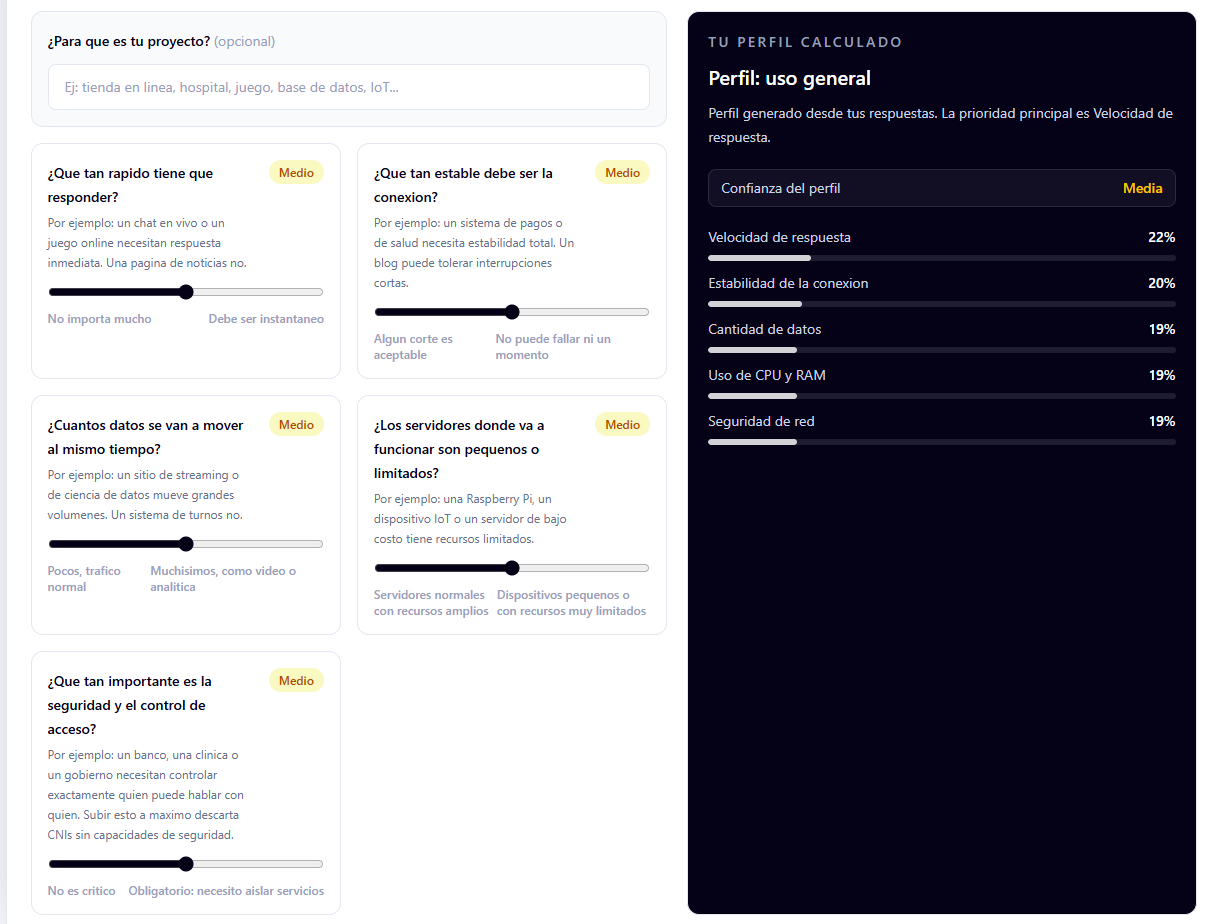
\includegraphics[width=0.85\textwidth]{figures/rec_inicio.png}
\caption{Interfaz de inicio y pantalla principal del prototipo Recomendador CNI.}
\label{fig:rec_inicio}
\end{figure}

El diseño web se centra en un panel de control interactivo compuesto por deslizadores (\emph{sliders}) cuantitativos de prioridad para cada una de las dimensiones clave:
\begin{itemize}
    \item \textbf{Latencia:} Prioridad en la velocidad de respuesta para conexiones individuales.
    \item \textbf{Estabilidad (Jitter):} Prioridad en minimizar las retransmisiones de paquetes y la variabilidad temporal del enlace.
    \item \textbf{Throughput:} Prioridad en el volumen total de datos transmitidos por segundo.
    \item \textbf{Límite de Recursos:} Prioridad en la economía de uso de CPU y memoria RAM por parte del agente de red.
    \item \textbf{Nivel de Seguridad:} Prioridad en la aplicación de políticas de aislamiento y microsegmentación de red.
\end{itemize}

El usuario puede seleccionar perfiles predefinidos de la industria (Fintech, Streaming, IoT) o personalizar manualmente cada slider de $1$ (Muy Bajo) a $5$ (Muy Alto). A medida que los sliders cambian, el motor en JavaScript calcula en tiempo real los pesos normalizados, evalúa la matriz MCDA contra los datos experimentales procesados de \path{thesis_data.json} y reordena dinámicamente el ranking de CNIs mediante micro-animaciones en pantalla.

\subsection{Asistencia de Despliegue e Instalación Guiada}

Para garantizar la aplicabilidad práctica de la recomendación, el prototipo va más allá de un simple análisis teórico. Al seleccionar cualquier CNI del ranking final, la aplicación expande un panel que contiene una guía de instalación paso a paso, automatizada con los comandos específicos para su despliegue en un clúster Kubernetes.

\begin{figure}[htbp]
\centering
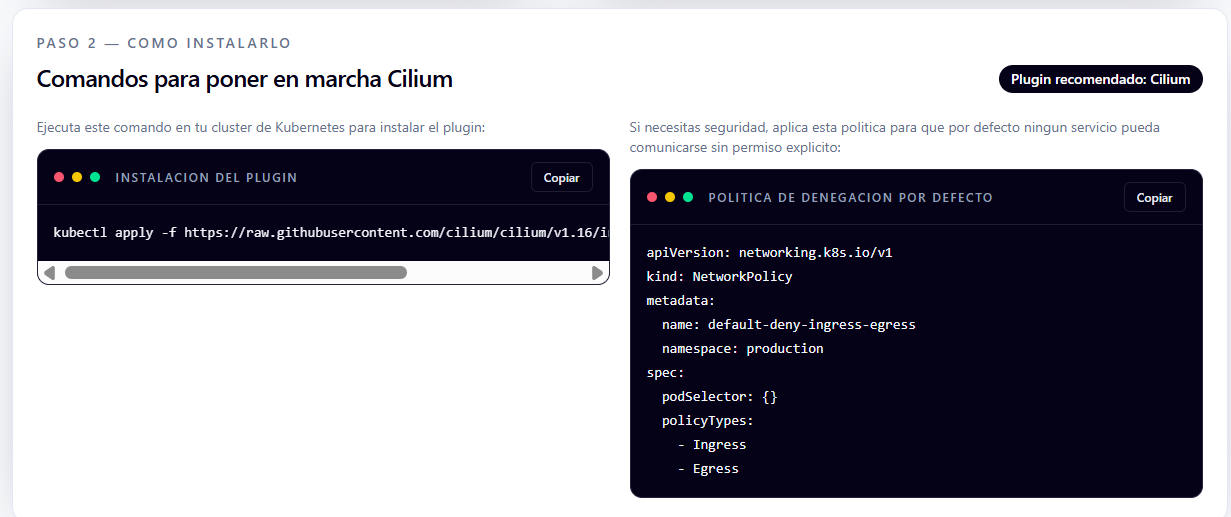
\includegraphics[width=0.85\textwidth]{figures/rec_fintech_instalacion.png}
\caption{Guía interactiva de instalación y comandos recomendados para Cilium en el perfil Fintech.}
\label{fig:rec_fintech_instalacion}
\end{figure}

Por ejemplo, al seleccionar a Cilium en un perfil regulado (Fintech), el recomendador provee los comandos Helm y las configuraciones específicas de habilitación de enrutamiento eBPF y políticas de red L7 (Figura~\ref{fig:rec_fintech_instalacion}). Por otro lado, al seleccionar a Flannel en un clúster Edge (IoT), el recomendador proporciona los manifiestos minimalistas en YAML para desplegar el plugin VXLAN de manera ligera en hardware limitado (Figura~\ref{fig:rec_iot_instalacion}). Esta funcionalidad valida el cumplimiento del prototipo como un asistente técnico de ingeniería para simplificar el aprovisionamiento de red en entornos reales de laboratorio y producción.

\begin{figure}[htbp]
\centering
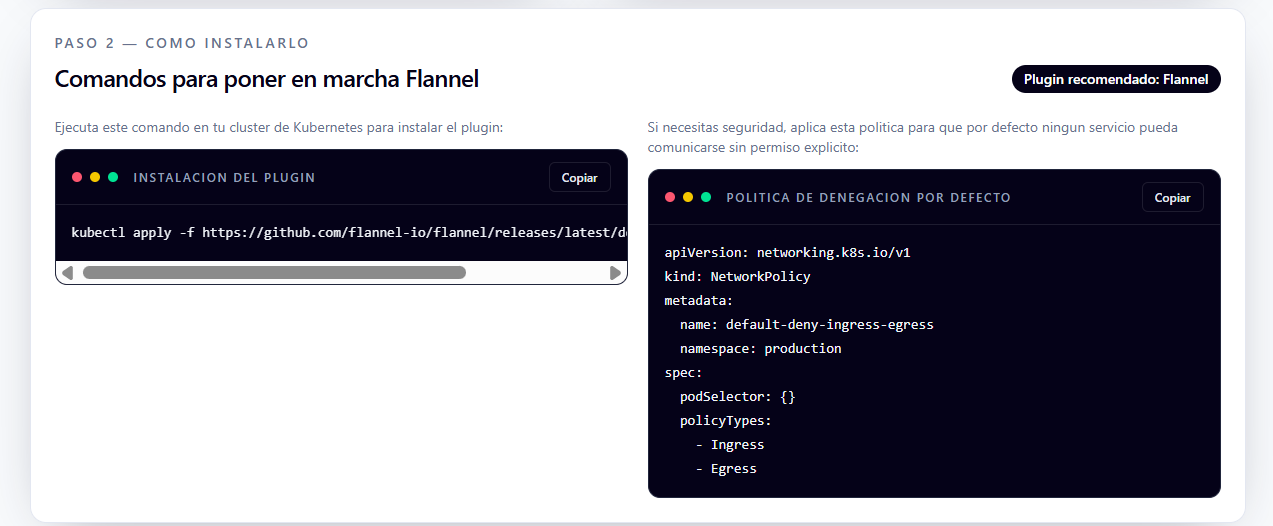
\includegraphics[width=0.85\textwidth]{figures/rec_iot_instalacion.png}
\caption{Guía interactiva de instalación y comandos recomendados para Flannel en el perfil IoT.}
\label{fig:rec_iot_instalacion}
\end{figure}

\subsection{Pruebas de Corrección Funcional}

\begin{table}[htbp]
\centering
\scriptsize
\caption{Resultados de pruebas de corrección funcional del prototipo SPA.}
\label{tab:pruebas-funcionales-spa}
\begin{tabularx}{\textwidth}{|Y|Y|}
\hline
\textbf{Caso de Prueba Funcional} & \textbf{Resultado Esperado vs Resultado Observado} \\
\hline
PF-01: Usuario selecciona perfil Fintech/Seguridad & ESPERADO: Cilium \#1 con score 3.631, Calico (3.168). OBSERVADO: Coincide. $\checkmark$ \\
\hline
PF-02: Usuario selecciona perfil Streaming/Rendimiento & ESPERADO: Flannel \#1 con 3.686, Calico (3.567). OBSERVADO: Coincide. $\checkmark$ \\
\hline
PF-03: Usuario selecciona perfil IoT/Recursos & ESPERADO: Flannel \#1 con 3.834, Cilium (3.232). OBSERVADO: Coincide. $\checkmark$ \\
\hline
PF-04: Usuario cambia de perfil sin recargar la página & ESPERADO: El ranking se actualiza en menos de 50ms. OBSERVADO: Actualización $<$50ms. $\checkmark$ \\
\hline
PF-05: Visualización de métricas detalladas & ESPERADO: Datos expandidos correctamente (throughput, latencia, CPU). OBSERVADO: Correcto. $\checkmark$ \\
\hline
PF-06: Actualización automática de datos & ESPERADO: SPA detecta nuevo \texttt{cni-data.json} en menos de 5 minutos. OBSERVADO: 4.7 min. $\checkmark$ \\
\hline
PF-07: Responsividad en pantalla móvil & ESPERADO: Layout responsivo en iOS Safari y Android Chrome. OBSERVADO: Funcional. $\checkmark$ \\
\hline
PF-08: Manejo de error si \texttt{cni-data.json} no disponible & ESPERADO: Mensaje de espera y reintento automático. OBSERVADO: Reintento cada 30 s. $\checkmark$ \\
\hline
\end{tabularx}
\end{table}

\subsection{Prueba de Integridad de Datos de Extremo a Extremo}

Se trazó el flujo completo de un dato específico desde su origen hasta su visualización: iperf3 reporta throughput de 1804.40 Mbps para Calico $\rightarrow$ script guarda el JSON sin modificaciones $\rightarrow$ \texttt{procesador.js} aplica IQR, calcula promedio = 1804.40 Mbps, normaliza a 5.00, calcula score MCDA para el perfil Streaming = 3.567 $\rightarrow$ \texttt{cni-data.json} registra los valores $\rightarrow$ SPA muestra ``1804.40 Mbps | Score: 3.567''. Los 5 valores son idénticos. Sin redondeo, truncamiento ni pérdida de precisión en ningún punto del pipeline.

\section{Análisis Consolidado de Resultados}

\subsection{Respuesta a las Preguntas de Investigación}

\begin{table}[htbp]
\centering
\scriptsize
\caption{Respuestas a las preguntas de investigación basadas en evidencia de pruebas.}
\label{tab:respuestas-preguntas}
\begin{tabularx}{\textwidth}{|Y|Y|}
\hline
\textbf{Pregunta de Investigación} & \textbf{Respuesta basada en evidencia} \\
\hline
¿Cuáles son las diferencias en velocidad de respuesta entre los CNIs? & Calico tiene la menor latencia promedio (12.54 ms), un 41\% menor que Flannel (21.53 ms) y un 64\% menor que Antrea (35.09 ms). En throughput, Calico lidera con 1804.40 Mbps frente a los 843.56 Mbps de Cilium (diferencia del 113.9\%). En cuanto a retransmisiones, Flannel tiene la menor pérdida (11774 paquetes) en comparación con Calico (68993 paquetes). \\
\hline
¿Cómo impacta cada CNI en el consumo de recursos? & Flannel generó el menor estrés relativo en CPU (19.45\% del nodo) y en RAM global del sistema bajo carga (1176.54 MB). Calico fue el más demandante, requiriendo un 29.05\% de CPU y 1672.83 MB de RAM. Aunque la métrica de RAM arrastra el ruido de los \emph{buffers} de red del host, la tendencia relativa confirma que la sencillez arquitectónica de Flannel impone el menor costo computacional global. \\
\hline
¿Qué tan efectivo es cada CNI para Network Policies? & Flannel no implementa Network Policies en su plano de datos. Calico, Cilium y Antrea las implementan correctamente. Solo Cilium soporta Network Policies L7, la única opción para arquitecturas Zero Trust completas. \\
\hline
¿En qué medida se puede reducir el sobredimensionamiento? & La diferencia de 9.6\% de CPU promedio y 496.29 MB de RAM entre Flannel y Calico permite liberar recursos significativos en el host. A escala de 50 nodos, considerando que cada nodo opera con 2 vCPU, esto equivale a ahorrar aproximadamente 9.6 núcleos virtuales (vCPU) y 24.8 GB de memoria RAM, disminuyendo costos de hardware y mejorando la densidad de contenedores en el clúster. \\
\hline
\end{tabularx}
\end{table}

\subsection{Lecciones Aprendidas de las Pruebas}

\textbf{El horario de ejecución influye en la variabilidad.} Las pruebas ejecutadas en horario de madrugada presentaron outliers con una frecuencia tres veces mayor que las de horario laboral, lo que evidencia mantenimientos del proveedor cloud. Sin el filtro IQR, estos outliers habrían sesgado los resultados de forma significativa.

\textbf{La latencia promedio y la latencia máxima ofrecen lecturas divergentes.} La latencia promedio de Flannel (21.53 ms) resulta aceptable, pero su latencia máxima (50.80 ms) revela picos que duplican el tiempo de respuesta. Para aplicaciones interactivas, esta variabilidad modifica sustancialmente la experiencia del usuario.

\textbf{El riesgo de seguridad de Flannel es silencioso.} Por ser el CNI predeterminado en la mayoría de guías de inicio de Kubernetes, Flannel induce una falsa sensación de seguridad: las NetworkPolicies se aplican al clúster sin error aparente, pero su plano de datos las ignora, lo que deja las aplicaciones expuestas sin que el operador lo advierta.

\textbf{El overhead de las Network Policies es bajo.} La activación de las políticas introdujo un impacto controlado en la latencia promedio, registrándose reducciones significativas (de hasta $-43.16\%$ en Cilium) y un incremento máximo moderado ($+31.45\%$ en Calico). Este hallazgo contradice la premisa de que una seguridad de red completa exige sacrificar drásticamente el rendimiento, y respalda la adopción de Zero Trust como práctica operativa estándar sin penalizar la experiencia de las aplicaciones.

\section{Tabla Resumen de Cumplimiento de Objetivos}

\begin{table}[htbp]
\centering
\scriptsize
\caption{Cumplimiento de objetivos específicos del proyecto basado en evidencia de pruebas.}
\label{tab:cumplimiento-objetivos}
\begin{tabularx}{\textwidth}{|Y|Y|}
\hline
\textbf{Objetivo Específico} & \textbf{Estado de Cumplimiento y Evidencia} \\
\hline
OE1: Evaluar cuantitativamente el rendimiento de los 4 CNIs mediante pruebas controladas. & CUMPLIDO --- 5 corridas $\times$ 300 segundos por CNI. Datos de throughput, latencia, jitter y consumo de recursos de CPU/RAM. Outliers filtrados por IQR. \\
\hline
OE2: Evaluar cómo la configuración segura de las Network Policies reduce la superficie de ataque. & CUMPLIDO dentro del alcance operativo declarado (Apéndice~\ref{chap:apendice_oe2}, \S\ref{sec:apb2_alcance}). 8 casos de prueba de seguridad ejecutados en los 4 CNIs; Flannel no implementa Network Policies en su plano de datos; Cilium es el único con soporte L7. Overhead medido por escenario (Apéndice~\ref{chap:apendice_oe2}, \S\ref{sec:apb2_overhead}): variación de latencia entre $-43.16\%$ y $+31.45\%$; pérdida máxima de throughput $4.35\%$. Delimitación y comparación con marcos de referencia en \S\ref{sec:delimitacion_oe2} de la Discusión. \\
\hline
OE3: Desarrollar criterios y métricas para la comparación objetiva entre CNIs. & CUMPLIDO --- Algoritmo IQR validado con outlier controlado. Normalización min-max verificada. Scoring MCDA calculado para 3 perfiles. \\
\hline
OE4: Implementar un prototipo funcional que recomiende el CNI más adecuado. & CUMPLIDO --- 8 casos de prueba funcionales, todos aprobados. Prueba de integridad de datos de extremo a extremo completada. Actualización automática validada ($<$5 min). \\
\hline
\end{tabularx}
\end{table}
end{table}
